\section{Conceptual Framework -- Variables and Hierarchy}\label{conceptual-framework-variables-and-hierarchy}

To understand how to use the utility bill calculation portion of EnergyPlus you first need to understand some important concepts of variables and hierarchy. A variable, for the purposes of this section, is simply a named holder of a series of numbers. In most cases, the variable will be a named holder of 12 numbers, one number for each monthly utility bill. Here is a visualization of a variable called Electric Energy Use:

% table 35
\begin{longtable}[c]{@{}ll@{}}
\caption{Example Electric Energy Use (for Economics Calculation) \label{table:example-electric-energy-use-for-economics}} \tabularnewline
\toprule 
Month & Electric Energy Use \tabularnewline
\midrule
\endfirsthead

\caption[]{Example Electric Energy Use (for Economics Calculation)} \tabularnewline
\toprule 
Month & Electric Energy Use \tabularnewline
\midrule
\endhead

January & 12143 \tabularnewline
February & 13454 \tabularnewline
March & 14178 \tabularnewline
April & 14876 \tabularnewline
May & 15343 \tabularnewline
June & 16172 \tabularnewline
July & 16105 \tabularnewline
August & 15762 \tabularnewline
September & 14543 \tabularnewline
October & 13987 \tabularnewline
November & 13287 \tabularnewline
December & 12403 \tabularnewline
\bottomrule
\end{longtable}

If you have ever done any computer programming, you can think of a variable as an array. Many of the names used in the utility bill calculation portion of EnergyPlus are names of variables. In the case of the UtilityCost:Charge objects, the name of the object is also used as a name of a variable.

In many of today's utility rates, the charges for energy or demand are broken into distribution and supply charges. To allow for this, more than one charge may to be defined for a particular category. The variables assigned to the same category are added together.

The categories are combined in following hierarchy:

\begin{figure}[hbtp] % fig 162
\centering
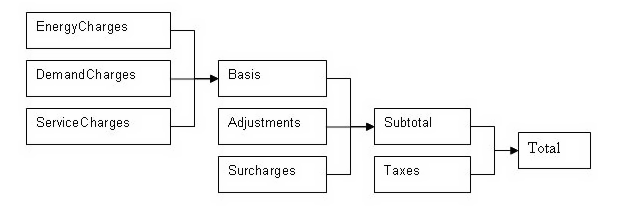
\includegraphics[width=0.9\textwidth, height=0.9\textheight, keepaspectratio=true]{media/image615.png}
\caption{Hierarchy for Economics Charges \protect \label{fig:hierarchy-for-economics-charges}}
\end{figure}

Any charges included in the EnergyCharges category are added together. The EnergyCharges, DemandCharges and ServiceCharges are added together to form the Basis. The Basis, Adjustments and Surcharges are added together to form the Subtotal. The Subtotal and Taxes are added together to be the Total. The total represents the total monthly charges on that tariff for the energy source used. The combining of categories together is performed automatically unless the user specifies the UtilityCost:Computation. In addition, each category, which is also a variable, may be used as a source. For example, a tax that is 5\% of the subtotal would be shown as:

\begin{lstlisting}

UtilityCost:Charge:Simple,
    TaxOfFivePercent,        ! Charge Variable Name
    TariffExample1,          ! Tariff Name
    Subtotal,                ! Source Variable
    Annual,                  ! Season
    Taxes,                   ! Category Variable Name
    0.05;                    ! Cost Per Unit Value or Variable Name
\end{lstlisting}

As you can see, the UtilityCost:Charge:Simple and UtilityCost:Charge:Block objects do most of the ``work'' of computing the annual energy cost. The benefit of using this categorization is that totals of each category are shown in the output reports and it organizes the charges in the monthly calculations in a logical way that fits almost all tariffs. If no categorization is desired, theoretically, all charges could be assigned to the Total category. The categories themselves are simply variable names. Charges may also be assigned to the ``NotIncluded'' category if the result of the charge is used as an intermediate calculation and should not be included in the Total.

The rest of this section is divided into a reference of the objects and the fields, a set of examples, discussion of the reporting, and a description of Complex Tariff Modeling. For most tariffs, simply using a variety of UtilityCost:Charge:Simple's and UtilityCost:Charge:Block's will result in a good model but for some more complex tariffs, especially ones with complex block sizes, variables may be computed using a very simple programming language that may appear in the UtilityCost:Computation object. This will be described more in the Complex Tariff Modeling section.
